\documentclass[letter,abstract=true,titlepage]{scrartcl}

\usepackage[USenglish]{babel}
\usepackage[T1]{fontenc}
%\usepackage[ansinew]{inputenc}
\usepackage{lmodern}

\usepackage{setspace}
\onehalfspacing
\AfterTOCHead{\singlespacing}
\KOMAoptions{DIV=last}
\usepackage{geometry}
\geometry{letterpaper, portrait, margin=1in}
\usepackage[utf8]{inputenc}
\usepackage{listings}
\renewcommand{\lstlistingname}{Code}
\usepackage{xcolor}
%\usepackage{fancyhdr}
\usepackage{amsmath}
\usepackage{graphicx}
%opening
\usepackage{scrlayer-scrpage}
\pagestyle{scrheadings}

\usepackage{xpatch}
\usepackage{lipsum}
\usepackage{indentfirst}

\usepackage{lmodern}

% (2) specify encoding
\usepackage[T1]{fontenc}

% (3) load symbol definitions
\usepackage{textcomp}
%\usepackage{underscore}

\usepackage{placeins}

\let\Oldsection\section
\renewcommand{\section}{\FloatBarrier\Oldsection}

\let\Oldsubsection\subsection
\renewcommand{\subsection}{\FloatBarrier\Oldsubsection}

\let\Oldsubsubsection\subsubsection
\renewcommand{\subsubsection}{\FloatBarrier\Oldsubsubsection}

\makeatletter
\xpatchcmd{\@addmargin}
{\setlength{\itemindent}{\z@}%
}
{\ifx\@afterindentfalse\@afterindenttrue
    \setlength{\itemindent}{\parindent}%
    \else
    \setlength{\itemindent}{\z@}%
    \fi}
{\typeout{Success patching}}{\typeout{Error patching}}
\makeatother

%\pagestyle{fancy}
%\fancyhf{}
%\rhead{EGR 680, Project \#1}
%\lhead{Scott Zuidema}
%\rfoot{Page \thepage}

\definecolor{mGreen}{rgb}{0,0.1,0}
\definecolor{mGray}{rgb}{0,0.2,0}
\definecolor{mPurple}{rgb}{0,0.3,0}
\definecolor{backgroundColour}{rgb}{0.95,0.95,0.95}

\lstdefinestyle{CStyle}{
    backgroundcolor=\color{backgroundColour},   
    commentstyle=\color{mGreen},
    keywordstyle=\color{mPurple},
    numberstyle=\color{mGray},
    stringstyle=\color{mPurple},
    basicstyle=\footnotesize,
    breakatwhitespace=false,         
    breaklines=true,                 
    captionpos=t,                    
    keepspaces=true,                 
    numbers=left,                    
    numbersep=5pt,                  
    showspaces=false,                
    showstringspaces=false,
    showtabs=false,                  
    tabsize=2,
    language=C
}

\lstdefinestyle{CStyle-tiny}{
    backgroundcolor=\color{backgroundColour},   
    commentstyle=\color{mGreen},
    keywordstyle=\color{mPurple},
    numberstyle=\tiny\color{mGray},
    stringstyle=\color{mPurple},
    basicstyle=\tiny,
    breakatwhitespace=false,         
    breaklines=true,                 
    captionpos=t,                    
    keepspaces=true,                 
    numbers=left,                    
    numbersep=5pt,                  
    showspaces=false,                
    showstringspaces=false,
    showtabs=false,                  
    tabsize=2,
    language=C
}


\lstdefinestyle{VerilogStyle-tiny}{
    backgroundcolor=\color{backgroundColour},   
    commentstyle=\color{mGreen},
    keywordstyle=\color{mPurple},
    numberstyle=\tiny\color{mGray},
    stringstyle=\color{mPurple},
    basicstyle=\tiny,
    breakatwhitespace=false,         
    breaklines=true,                 
    captionpos=t,                    
    keepspaces=true,                 
    numbers=left,                    
    numbersep=5pt,                  
    showspaces=false,                
    showstringspaces=false,
    showtabs=false,                  
    tabsize=2,
    language=Verilog
}
\lstdefinestyle{VerilogStyle}{
    backgroundcolor=\color{backgroundColour},   
    commentstyle=\color{mGreen},
    keywordstyle=\color{mPurple},
    numberstyle=\color{mGray},
    stringstyle=\color{mPurple},
    basicstyle=\footnotesize,
    breakatwhitespace=false,         
    breaklines=true,                 
    captionpos=t,                    
    keepspaces=true,                 
    numbers=left,                    
    numbersep=5pt,                  
    showspaces=false,                
    showstringspaces=false,
    showtabs=false,                  
    tabsize=2,
    language=Verilog
}
\author{Permformed by: Student A\\Student B}
\rohead{Student A\\Student B}
\lohead{EGR 227-xx Labs \#y}
%\titlehead{Grand Valley State University}
\title{Laboratory Z}
\subtitle{Title for Your Laboratory}
\subject{EGR 227-xx\\Semester X\\Prof. Y}
\author{Student A\\Student B}

\begin{document}
 
\maketitle
\section{Introduction}
Place an introduction to the laboratory here.

\section{Tools Used}
\begin{itemize}
\item Laptop (Linux OS)
\item STM32L053 Nucleo Board
\item VSCode 1.62.0
\item Breadboard
\end{itemize}

\section{Procedure}
Discuss the steps needed to recreate the laboratory.\\

Include a figure of your laboratory to demonstrate setup.  See Figure \ref{fig:example_setup} on page \pageref{fig:example_setup} for an example of how to reference a figure.

\begin{center}
    \begin{figure}[h!]
        \centering
        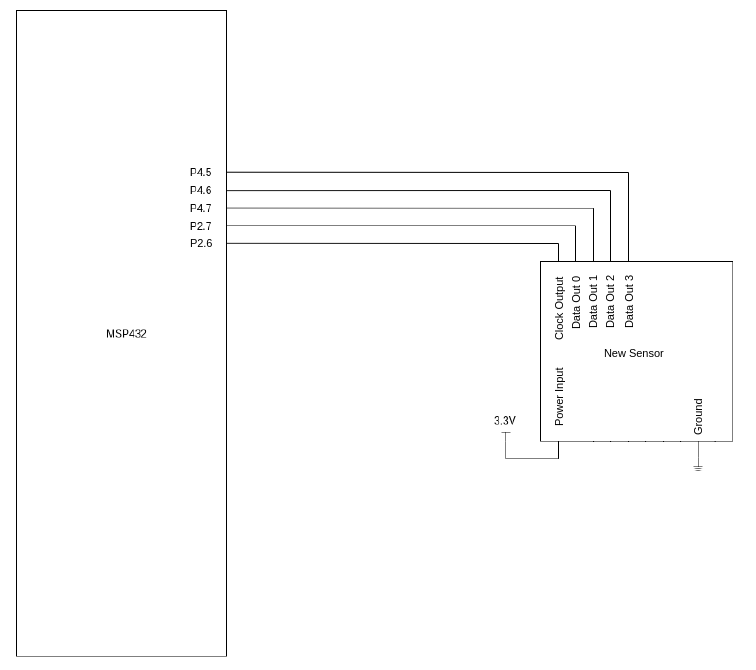
\includegraphics[width=0.9\textwidth]{images/MSP432_Blackbox_Communication.png}
        \caption{Example figure of the setup of the microcontroller}
        \label{fig:example_setup} 
    \end{figure}
\end{center} 

This is an example equation.  Equation \ref{eq:example_equation} on page \pageref{eq:example_equation} is an equation that does stuff.\\
\begin{equation}\label{eq:example_equation}
    K_{k}=P_{k|k-1}+H_k^TS_k^{-1}
\end{equation}

If an important part of your code exists you want to reference, you can reference a portionf of a main file like this.  A useful function to use during this procudure is shown in Code \ref{code:main.c_start}.  It is recommended to approach the code in this way to improve efficiency.\\

\lstinputlisting[linerange={1-4},label={code:main.c_start},caption={Beginning of main.c Code for \@title : \@subtitle},style=CStyle-tiny]{../Core/Src/main.c}



\section{Results}
The completed code for this laboratory is shown in the Appendix in Code \ref{code:main.c} on page \pageref{code:main.c}.\\

The output from running the C code shown in Code \ref{code:main.c} on the system show in Figure \ref{fig:example_setup} on page \pageref{fig:example_setup} is shown below:\\
% \lstinputlisting[label={code:output},caption={Output of running system Encryption},style=CStyle-tiny]{Output}

Include a picture of the laboratory running successfully.\\

\section{Conclusion}
This lab was completed successfully.  If the laboratory was expanded upon to add additional features, these are the things recommended adding.  If the laboratory was to be repeated, it is recommended that the next attempt keep these things in mind while performing the lab.

\newpage
\section{Appendix}

\lstinputlisting[label={code:main.c},caption={main.c Code for \@title : \@subtitle},style=CStyle-tiny]{../Core/Src/main.c}

\end{document}
